\section{Experimentos}

\begin{frame}{Experimentos}
\begin{alertblock}{Experimentos}
\end{alertblock}
\end{frame}

%*******************************************************************
\begin{frame}{Experimento 1: Verificação autoral}
\fontsize{3.0mm}{4.0mm}\selectfont
\begin{block}{Publicação 1}
	CUSTÓDIO, J. E.; PARABONI, I. Similaridade de Textos aplicada à Verificação Autoral.
	In: 1st International Congress on Digital Humanities in Rio de Janeiro. [S.l.]: Fundação
	Getúlio Vargas, 2018.
\end{block}

\begin{block}{Verificação autoral ou atribuição por similaridade}
	\begin{itemize}
		\item Deseja-se saber se pares de documentos foram escritos pelo mesmo autor. \cite{Koppel2012}
		\item Aplicável quando não se sabe quem são os autores.
		\item Modelo supervisionado por vizinho mais próximo.
		\begin{itemize}\selectFont
			\item O documento é atribuído ao vizinho mais próximo.
			\item A distância pode ser usada no agrupamento autoral.
		\end{itemize}
		\item Modelo transformado
		\begin{itemize}\selectFont
			\item Documentos são uma representação única.
		\end{itemize}
	\end{itemize}
\end{block}
\end{frame}

\begin{frame}{Experimento 1: Verificação autoral}
\begin{block}{Extração de características}
Modelo de espaço de vetores (BOW) com n-gramas de caracteres normalizados com norma L1 (TF).\\
Foram selecionadas os n-gramas presentes em 90\% do córpus ({\it Common n-grams} \cite{Keselj2003}).
\end{block}
\begin{block}{Distâncias}
Medidas de similaridade textual entre os documentos A e B do córpus C:

\begin{equation}
Cossenos \left ( A,B \right )= \frac{A\cdot B}{\left \| A \right \| \left \| B \right \|}
\label{eq:cosseno}
\end{equation}

\begin{equation} 
Jaccard(A,B) = \frac{\left | A \cap B \right |}{\left | A \cup B \right |}
\label{eq:jaccard}
\end{equation}

%		\begin{equation}
%		Keselj(A,B) = \sum \left ( \frac{ 2*\left(A-B \right ) }{A+B}\right )^{2}
%		\label{eq:keselj}
%		\end{equation}


\begin{equation}
Stamatatos(A,B, N) = \sum_{i} \left ( \frac{ 2*\left(A-B \right ) }{A+B}\right )^{2} * \left ( \frac{ 2*\left(A-C \right ) }{A+C}\right )^{2}
\label{eq:stamatatos}
\end{equation}
\end{block}
\end{frame}

\begin{frame}{Experimento 1: Verificação autoral}
Análise da capacidade de separação da medidas de similaridade aplicadas córpus PAN-CLEF 2014 \cite{aa-overview-2014}

\begin{columns}
\begin{column}{0.60\textwidth}
\begin{figure}[]\selectFont
	\centering
	\caption{\selectFont Diagnósticos}
	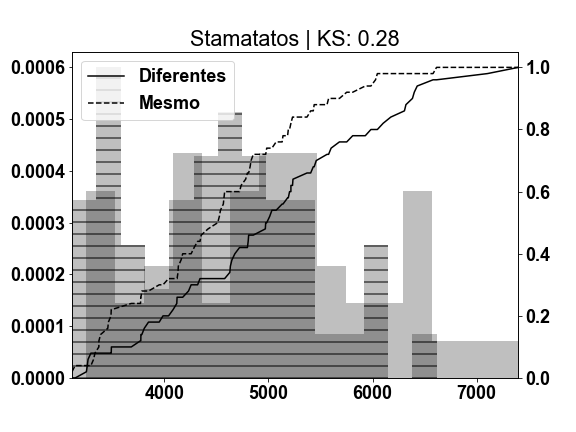
\includegraphics[width=.45\textwidth]{experimentoVerificacao/HDRIO_KS_spanish_Stamatatos.png} \vspace{0.3cm}
	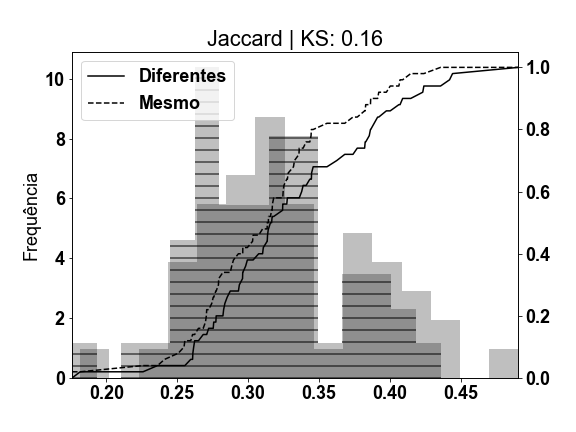
\includegraphics[width=.45\textwidth]{experimentoVerificacao/HDRIO_KS_spanish_Jaccard.png} \vspace{0.3cm}
	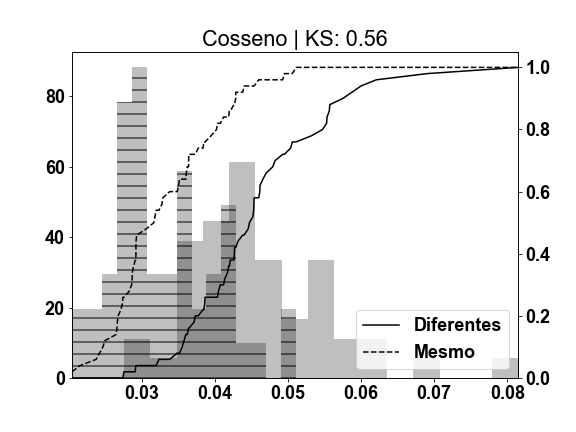
\includegraphics[width=.45\textwidth]{experimentoVerificacao/HDRIO_KS_spanish_Cosseno.png}
	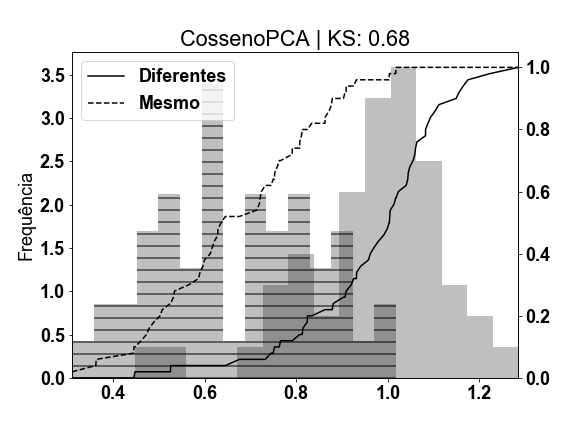
\includegraphics[width=.45\textwidth]{experimentoVerificacao/HDRIO_KS_spanish_CossenoPCA.png}
	\label{fig:exemplo}
\end{figure}
\end{column}
\begin{column}{0.37\textwidth}

\begin{itemize}
	\item Histograma para mesma autoria (tracejado).
	\item Histograma para autorias diferentes (liso).
	\item Distribuição acumuladas (linhas).
	\item Separação pela métrica Kolmogorov-Smirnov.
	\item Métricas AUC e acurácia.
\end{itemize}
\end{column}
\end{columns}


\end{frame}
\begin{frame}{Experimento 1: Verificação autoral}
	\begin{block}{Modelo proposto 1 - MP1}
	\begin{itemize}
		\item As distâncias foram utilizadas como variáveis para o modelo.
		\item Aplicado a normalização minmax.
		\item Aplicado a regressão logística.
		\end{itemize}
	\end{block}
	\begin{block}{Modelo proposto 2 - MP2}
		\begin{itemize}
		\item Os documentos conhecidos $C$ e de autoria desconhecidas $D$ foram unificados em um úncio BoW através da equação:
		\begin{equation}
		MP2\left ( C_{ij}, D_{ij} \right ) = \log\left ( 1 + \frac{\left ( C_{ij}-D_{ij} \right )^2}{C_{ij}+1} \right )
		\label{eq:verificacao.mp2}
		\end{equation}
		\item Aplicado a normalização minmax.
		\item Aplicado a regressão logística.
		\end{itemize}		
	\end{block}	
\end{frame}

\begin{frame}{Experimento 1: Verificação autoral}
	\begin{table}[]
	\caption{Verificação autoral - Resultados médios das métricas AUC e acurácia em 5-partições.}\selectFont
	\begin{tabular}{l|cc|cc}
		\toprule
		\multirow{2}{*}{\bf Modelo} & \multicolumn{2}{c|}{\bf PAN2014 (EE e EM)} & \multicolumn{2}{c}  {\bf PAN2014{-}SP} \\ \cline{2-5}
		                            & {\bf ROC}  &        {\bf Acurácia}         & {\bf ROC}  &      {\bf Acurácia}       \\ \hline
		Jaccard                     &    0,60    &             0,56              &    0,57    &           0,52            \\
		Cossenos                    &    0,63    &             0,50              &    0,88    &           0,77            \\
		Cossenos\_PCA               &    0,63    &             0,55              & {\bf 0,92} &        {\bf 0,83}         \\
		Keselj                      &    0,61    &             0,54              &    0,71    &           0,60            \\
		Stamatatos                  &    0,60    &             0,55              &    0,59    &           0,54            \\ \hline
		MP1 – Mix                   & {\bf 0,75} &          {\bf 0,67}           &    0,72    &           0,62            \\
		MP2 – BOW                   &    0,62    &             0,53              & {\bf 0,93} &        {\bf 0,85}         \\ \bottomrule
	\end{tabular} 
	\label{tab.results.verificacao}
	%\SourcePadrao
\end{table}

{\selectFont
PAN2014 (EE e EM) córpus com textos em língua inglesa, PAN2014{-}SP textos em língua espanhola.
}
\end{frame}


%*******************************************************************
\begin{frame}{Experimento 2: Atribuição Autoral}
	\begin{block}{Publicação 2}
		CUSTÓDIO, J. E.; PARABONI, I. EACH-USP Ensemble Cross-domain Authorship
		Attribution: Notebook for PAN at CLEF 2018. In: CAPPELLATO, L. et al. (Ed.).
		Working Notes Papers of the CLEF 2018 Evaluation Labs. [S.l.]: CLEF and CEUR-WS.org,
		2018. (CEUR Workshop Proceedings). ISSN 1613-0073.
	\end{block}
	
	\begin{block}{Atribuição por aprendizado de máquina supervisionado}
	\begin{itemize}
		\item Tem-se um conjunto de documentos para os quais se sabe quem são os autores e um documento do qual deseja-se atribuir.
		\item O classificador extrai a ``assinatura do estilo''.
		\item Aspectos inconscientes, como a sintaxe, são mais importantes que a semântica.
		\item O trabalho apresentado foi parte da participação da tarefa de AA da competição PAN-CLEF2018.
	\end{itemize}
	\end{block}
\end{frame}
	
\begin{frame}{Experimento 2: Atribuição Autoral}
	\begin{block}{Baseline {\it Bas.PAN}}
		Os organizadores forneceram um sistema {\it baseline} pelos com as seguintes características:
		\begin{itemize}
			\item N-gramas de caracteres de tamanho fixo.
			\item Normalização no documento por TF.
			\item Sem normalização no córpus.
			\item Frequência mínima de 4 ocorrências.
			\item Classificador SVM encapsulado nas estratégias um-contra-um e um-contra-todos.
			\item Foi otimizado por {\it grid search} com validação cruzada com 5 partições, e os melhores parâmetros foram:
			\begin{itemize}\selectFont
				\item n-gramas de tamanho 4.
				\item Frequência mínima de 5 documentos.
				\item SVM com estratégia um-contra-todos.
			\end{itemize}
		\end{itemize}
	\end{block}
\end{frame}

\begin{frame}{Experimento 2: Atribuição Autoral}
	Dado nossas premissas, o sistema final PAN2018 para AA consistiu de um comitê que concatenou as fontes de informações em uma saída única.
	
	\begin{figure}[]\selectFont
	\caption{\selectFont Método proposto final}
	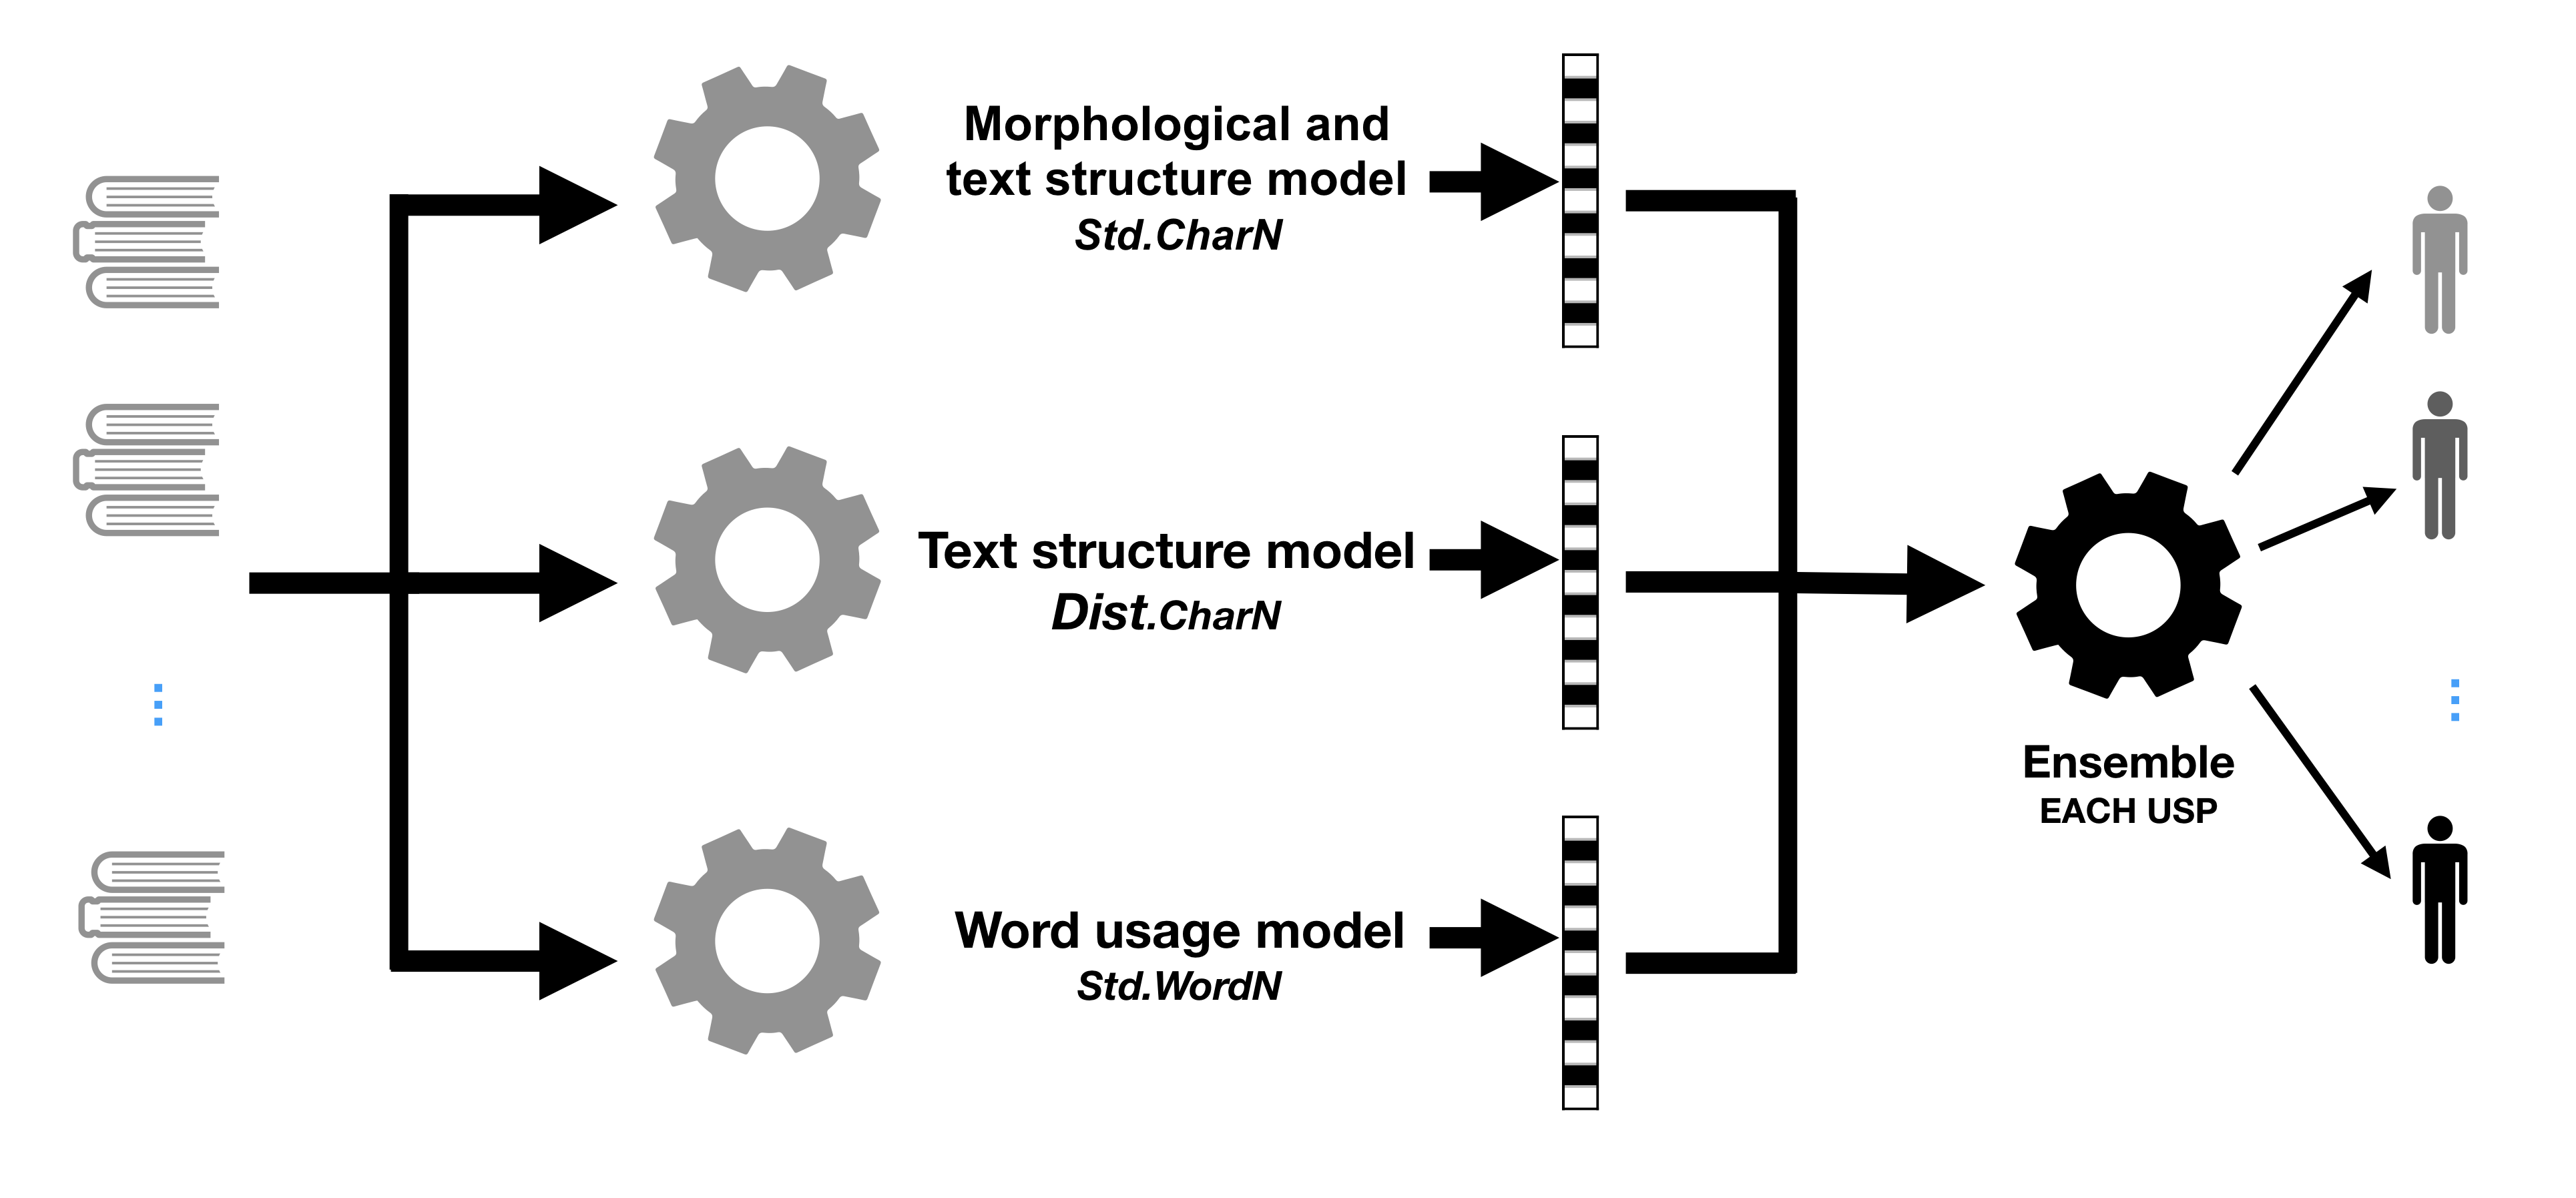
\includegraphics[width=.7\textwidth]{images/prop1_Diagramas.png}
	\end{figure}
	
	O sistema foi otimizado por {\it grid search} com validação cruzada de 5 partições.
	\end{frame}
	
	\begin{frame}{Experimento 2: Atribuição Autoral}
	Premissa: O estilo de escrita de autor pode ser capturado através de diversas fontes de informação, como sintática, léxica e semântica.
	\begin{block}{Método proposto {\it Std.word}}
	Consistiu de um modelo BOW de n-gramas de palavras tradicional.
	\end{block}
	\begin{block}{Método proposto {\it Std.char}}
	Consistiu de um modelo BOW de n-gramas de caracteres tradicional.
	\end{block}
	\begin{block}{Método proposto {\it Dist.char}}
	Consistiu de um modelo BOW de n-gramas de caracteres onde são letras maiúscula e minúsculas sem acento são distorcidas, deixando a pontuação, espaços e letras com diacríticos.
	\end{block}
\end{frame}

\begin{frame}{Experimento -  Modelo de distorção textual em caracteres}
	O modelo \textit{Dist.charN} utiliza distorção textual e foi inspirado em \citeonline{aa-distortion}. O objetivo da distorção é mascarar conteúdos que estariam se comportando como ruído para o modelo. \citeonline{aa-distortion} utiliza distorções para mascarar palavras menos frequentes, que estariam relacionadas ao tópico. O modelo \textit{Dist.charN} atua sobre carácter, filtrando a utilização de espaços, pontuação e caracteres com diacríticos, de forma a mascarar caracteres comuns, ou seja, letras minúsculas e maiúsculas. A tabela \ref{tb.Dist} ilustra a aplicação desse método.
	
	
	\begin{table}[ht]
		\centering
		\caption{Exemplo de distorção de texto aplicado o 1o. documento do 9o. problema da base de treinamento.}
		\begin{tabular}{m{5cm}m{5cm}}
			\toprule
			{\bf Texto original} & {\bf Texto transformado} \\ \hline
			\texttt{-¿Y cómo sabes que no lo ama? -Inglaterra se preguntó a su vez si habría un muñeco del esposo también. }
			&
			\texttt{-¿* *ó** ***** *** ** ** ***? -********** ** *******ó * ** *** ** ****í* ** **ñ*** *** ****** *****é*.} \\
			\bottomrule
		\end{tabular}
		\label{tb.Dist}
	\end{table}
\end{frame}

\begin{frame}{Experimento 2: Atribuição Autoral}
	\selectFont
	\setlength{\tabcolsep}{3pt}
	\begin{table}[!htbp]
		\centering
		\caption{\selectFont Valores ótimos encontrados para PAN2018}
		\begin{tabular}{m{2.2cm}m{4cm}m{4cm}}
		\toprule
		\textbf{Módulo} & \textbf{Parâmetros} & \textbf{Valores ótimos} \\ 
		\midrule
		\multirow{6}{2.2cm}{\bf Extração de características} & Faixa n-gram & 
		\begin{tabular}[c]{@{}l@{ - }l@{}}
			Std.charN  & Início=2 Fim=5 \\
			Dist.charN & Início=2 Fim=5 \\
			Std.WordN  & Início=1 Fim=3
		\end{tabular}\\ 
		& Freq. min. doc. & 0,05 \\ %\cline{2-3} 
		& Freq. max. doc. & 1,0 \\ %\cline{2-3} 
		& TF & Sublinear \\ %\cline{2-3} 
		& IDF & Suavizado \\ %\cline{2-3} 
		& Normalização no documento & L2 \\ 
		\hline
		{\bf Transformação} & PCA & 0,99 \\ 
		\bottomrule
		\end{tabular}
		\label{tab.optimal}
	\end{table}
\end{frame}

\begin{frame}{Experimento 2: Resultados obtidos em treinamento}
	\setlength{\tabcolsep}{4pt}\selectFont
	\begin{table}[!htbp]
	\centering
	\caption{\selectFont F1 para PAN-CLEF 2018 AA no córpus de desenvolvimento}
	\begin{tabular}{ccc ccccc}
		\bottomrule
		{Problema} & {Língua} & {Autores} & {Bas.PAN} & {Std.charN} & {Dist.charN} & {Std.wordN} &   {Comitê}   \\ \midrule
		    01     &    EN    &    20     & 0,514     &    0,609    &    0,479     &    0,444    & {\bf 0,625}  \\
		    02     &    EN    &     5     & 0,626     &    0,535    &    0,333     &    0,577    & {\bf 0,673}  \\
		    03     &    FR    &    20     & 0,631     &    0,681    &    0,568     &    0,418    & {\bf 0,776}  \\
		    04     &    FR    &     5     & 0,747     &    0,719    &    0,586     &    0,572    & {\bf 0,820}  \\
		    05     &    IT    &    20     & 0,529     &    0,597    &    0,491     &    0,497    & {\bf 0,578}  \\
		    06     &    IT    &     5     & 0,614     &    0,623    &    0,595     &    0,520    & {\bf 0,663}  \\
		    07     &    PL    &    20     & 0,455     &    0,470    &    0,496     &    0,475    &   { 0,554}   \\
		    08     &    PL    &     5     & 0,703     & {\bf 0,948} &    0,570     & {\bf 0,922} &    0,922     \\
		    09     &    ES    &    20     & 0,709     & {\bf 0,774} &    0,589     &    0,616    &    0,701     \\
		    10     &    ES    &     5     & 0,593     &    0,778    & {\bf 0,802}  &    0,588    & {\bf 0,830}  \\ \bottomrule
		  Média    &          &           & 0,612     &    0,673    &    0,551     &    0,563    & {\bf 0,714 } \\ \bottomrule
	\end{tabular}
	\label{tab.results}
	\end{table}
\end{frame}


\begin{frame}{Experimento 2: Resultados obtidos na PAN2018}
	\selectFont
	Resultado geral apresentados pelos organizadores do PAN2018 \cite{aa-overview-2018}.
	
	\setlength{\tabcolsep}{3pt}\selectFont
	\begin{table}[]
	\centering
	\caption{\selectFont PAN-CLEF 2018 - 3 melhores equipes - por língua}
	\begin{tabular}{m{5cm}cccccc}
		\toprule
		{\bf Equipe}                      & {\bf F1 Geral} &  {\bf EN}   &  {\bf FR}   &  {\bf IT}   & {\bf PL} &  {\bf ES}   \\ \midrule
		\citeonline{custodioParaboni2018} &  {\bf 0,685}   &    0,744    & {\bf 0,668} &    0,676    &  0,482   & {\bf 0,856} \\
		\citeonline{Murauer2018}          &     0,643      & {\bf 0,762} &    0,607    &    0,663    &  0,450   &    0,734    \\
		\citeonline{Halvani2018}          &     0,629      &    0,679    &    0,536    & {\bf 0,752} &  0,426   &    0,751    \\
		PAN18-BASELINE                    &     0,584      &    0,697    &    0,585    &    0,605    &  0,419   &    0,615    \\ \bottomrule
	\end{tabular}
	
	\caption{\selectFont PAN-CLEF 2018 - 3 melhores equipes - por língua}
	\begin{tabular}{m{5cm}cccc}
		\toprule
		{}                                &     \multicolumn{4}{c}{\bf Quantidade de autores}     \\ \cline{2-5}
		{\bf Equipe}                      &  {\bf 20 }  &  {\bf 15 }  &  {\bf 10 }  &  {\bf 5 }   \\ \midrule
		\citeonline{custodioParaboni2018} & {\bf 0,648} & {\bf 0,676} & {\bf 0,739} & {\bf 0,677} \\
		\citeonline{Murauer2018}          &    0,609    &    0,642    &    0,680    &    0,642    \\
		\citeonline{Halvani2018}          &    0,609    &    0,605    &    0,665    &    0,636    \\
		PAN18-BASELINE                    &    0,546    &    0,532    &    0,595    &    0,663    \\ \bottomrule
	\end{tabular}
	\label{tab.experimento1.resultados.por.autores}
	\end{table}
\end{frame}





\begin{frame}{Experimento -  Características mais importantes}
	\setlength{\tabcolsep}{15pt}\selectFont
	\begin{table}[h]
	\centering
	\caption{Características textuais mais relevantes para {\em Std.charN}}
	\label{tableTop.Std.charN}
	\begin{tabular}{c|c|c|c|c}
		\toprule
		         \multicolumn{5}{c}{\bf Candidatos}          \\ \hline
		{\bf 01} & {\bf 02} & {\bf 03} & {\bf 04} & {\bf 05} \\ \midrule
		\_as\_l  &  \_Sti   &  \_sub   &  \_joi   &  \_day,  \\
		  \_'    &  \_"Can  &  \_suc   &   \_gh   &  \_dev   \\
		 \_prec  &  \_"Ca   & \_I\_fi  &   \_er   &  \_dete  \\
		 \_I'd   &  \_"Be   &  \_succ  &  \_glow  &  \_plac  \\
		 \_"Are  &   \_K    &  \_subs  &   \_Is   &  \_mut   \\
		  \_Re   & \_but\_  &  \_I\_f  &  \_sta   &  \_must  \\
		 \_smel  &  \_Ofte  &   \_"T   &  \_gor   &  \_Dro   \\
		 \_leak  &  \_posi  &  \_a\_t  &  \_sorr  & \_day\_  \\
		\_is\_s  &  \_For   &  \_"St   & \_eat\_  & \_she\_  \\
		 \_spu   &   \_Ri   & \_a\_sw  & \_If\_t  &  \_chi   \\ \bottomrule
	\end{tabular}
	\end{table}
	{\selectFont Extraído do subconjunto 02 com textos em inglês e com 5 autores.}
\end{frame}

\begin{frame}{Experimento - Anexo: Características mais relevantes}
	\setlength{\tabcolsep}{15pt}\selectFont
	\begin{table}[h]
	\centering
	\caption{\selectFont Características textuais mais relevantes para {\em Dist.charN}}
	\label{tableTop.Std.distN}
	\begin{tabular}{c|c|c|c|c}
		\toprule
		         \multicolumn{5}{c}{\bf Candidatos}          \\ \hline
		{\bf 01} & {\bf 02} & {\bf 03} & {\bf 04} & {\bf 05} \\ \midrule
		 *\_‘**  & \_**\_-  &   "*'    & *\_\~\_  & *\_–\_*  \\
		 \_**-   & \_**\_(  &  "*\_**  &  *\_\~   &  '*,\_*  \\
		   *'    & \_**\_*  &  !),\_*  & *\_.\_*  &   "\_    \\
		  **).   &    *!    &   *!!    &   '***   &   *\_–   \\
		 **),\_  & \_**\_'  &  *'*\_*  &  '****   &  *\_–\_  \\
		*\_-\_*  &  *!\_*   &  **\_*'  &  "\_**'  &   '*.    \\
		 *\_-\_  &  *\_“**  &  **\_**  &  \_É***  &   \_“*   \\
		 \_'**   &  \_\~\_  &  **\_*’  &  \_“*’   &   \_-    \\
		  !),    & \_\~\_*  &  \_**!   &  \_**..  &  \_-\_   \\ \bottomrule
	\end{tabular}
	\end{table}
	{\selectFont Extraído do subconjunto 02 com textos em inglês e com 5 autores.}
\end{frame}

\begin{frame}{Experimento - Características mais relevantes}
	\setlength{\tabcolsep}{3pt}\selectFont
	\begin{table}[ht]
	\centering
	\caption{Características textuais mais relevantes em {\em Std.wordN}}
	\label{tableTop.Std.wordN}
	\begin{tabular}{c|c|c|c|c}
		\toprule
		                                \multicolumn{5}{c}{\bf Candidatos}                                 \\ \hline
		    {\bf 01}     &      {\bf 02}      &      {\bf 03}      &      {\bf 04}      &     {\bf 05}     \\ \midrule
		  about\_what    &    against\_his    &      an\_odd       &      although      & and\_pulled\_him \\
		and\_practically &    and\_it\_was    &   and\_then\_he    &      an\_eye       &   and\_pulling   \\
		    any\_of      &      and\_so       &    acknowledged    &     and\_said      &   across\_his    \\
		   any\_more     &    and\_already    &    and\_he\_had    &     and\_takes     &   across\_the    \\
		  and\_nearly    &     and\_steve     &     are\_your      &     and\_just      &     and\_all     \\
		  and\_pulled    &      and\_say      &     again\_to      &      ancient       &   against\_her   \\
		     agree       &       accent       &     and\_tell      &     amount\_of     &      among       \\
		   all\_tony     &      and\_wet      &     and\_forth     &       always       & about\_what\_to  \\
		       ah        &     apparently     &     are\_just      &    and\_grinned    &      acting      \\
		 and\_wet\_and   &       after        &   and\_grabbing    &     about\_the     &   about\_their   \\
		    %an\_arm     &        act         &     and\_give      & against\_the\_wall &    and\_tony     \\
		%and\_her\_eyes  &    and\_somehow    &       anyone       &  an\_arm\_around   &    and\_leave    \\
		    %all\_in     &  and\_said\_with   & against\_his\_skin &      and\_not      &    and\_left     \\
		   %after\_he    &      and\_was      &     and\_moved     &  are\_you\_saying  &     anymore      \\
		   %and\_knew    & against\_her\_skin &     appreciate     &     and\_took      &  and\_then\_she  \\
		    %anyway      &   and\_suddenly    &        aren        &   and\_the\_last   &   and\_looked    \\
		   %and\_had     &   and\_saw\_the    &      able\_to      &       allow        &    and\_began    \\
		  %an\_answer    &  and\_this\_time   &        all         &    ability\_to     &     and\_no      \\
		  %anticipate    &    along\_with     &    about\_being    &     all\_they      &      am\_so      \\
		   %all\_she     &        aid         &      answered      &    and\_turned     &     against      \\ \bottomrule
	\end{tabular}
	\end{table}
	{\selectFont Extraído do subconjunto 02 com textos em inglês e com 5 autores.}
\end{frame}
